\section{Problema 2}
\begin{tcolorbox}[colback=gray!15,colframe=gray!1!gray,title=Teorema 3.2 de \cite{rudin1976principles} ]
	Let $\left\{p_{n}\right\}$ be a sequence in a metric space $X$.
	\begin{enumerate}
		\item $\left\{p_{n}\right\}$ converges to $p \in X$ if and only if every neighborhood of $p$ contains all but finitely many of the terms of $\left\{p_{n}\right\}$
		\item If $p \in X, p^{\prime} \in X$, and if $\left\{p_{n}\right\}$ converges to $p$ and to $p^{\prime}$, then $p^{\prime}=p$.
		\item If $\left\{p_{n}\right\}$ converges, then $\left\{p_{n}\right\}$ is bounded.
		\item If $E \subset X$ and if $p$ is a limit point of $E$, then there is a sequence $\left\{p_{n}\right\}$ in $E$ such that $p=\lim _{n \rightarrow \infty} p_{n}$.
	\end{enumerate}
\end{tcolorbox}

Sean $X$ y $Y$ espacios métricos y sea $A$ un subconjunto no vacío de $X$. Si $f$ y $g$ son mapeos
continuos de $X$ en $Y$, tales que $f(x) = g(x)$, $\forall x\in A$, demuestre que $f(x) = g(x)$, $\forall \ x \in \overline{A} $.

\begin{proof}
	A probar: $f(x)=g(x), \ \forall \ x\in \overline{A}$. Observamos que el problema consiste: 
	\begin{center}
		
		
		\tikzset{every picture/.style={line width=0.75pt}} %set default line width to 0.75pt        
		
		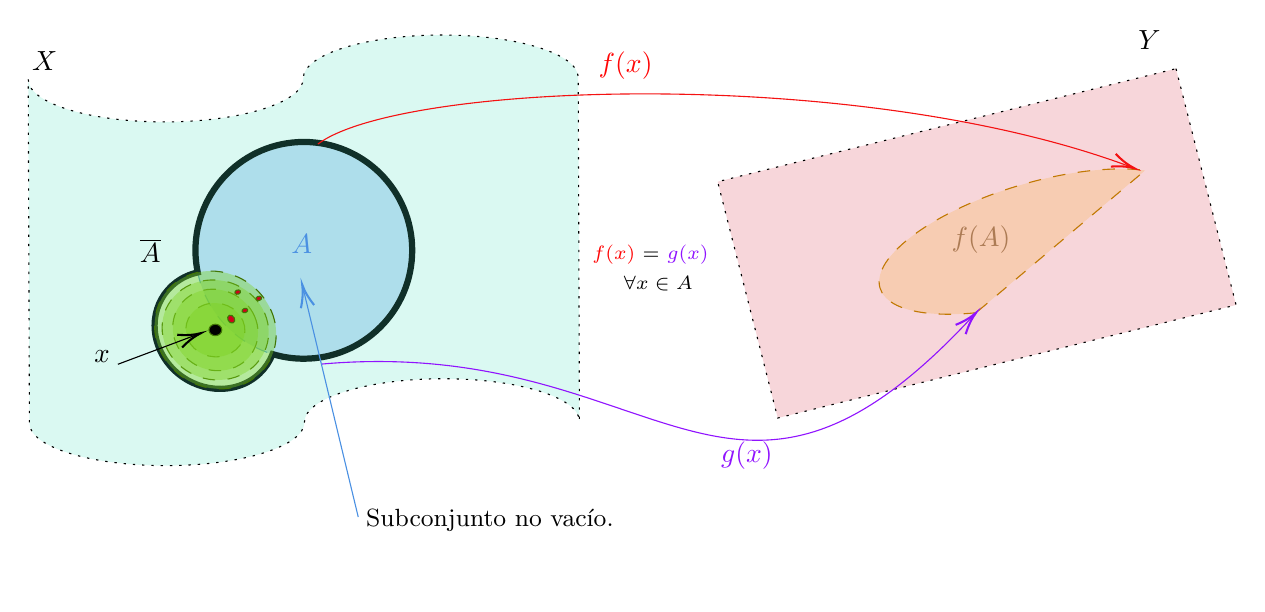
\begin{tikzpicture}[x=0.75pt,y=0.75pt,yscale=-1,xscale=1]
			%uncomment if require: \path (0,300); %set diagram left start at 0, and has height of 300
			
			%Shape: Circle [id:dp4460526059104589] 
			\draw  [color={rgb, 255:red, 74; green, 144; blue, 226 }  ,draw opacity=1 ][fill={rgb, 255:red, 74; green, 144; blue, 226 }  ,fill opacity=0.3 ][dash pattern={on 4.5pt off 4.5pt}] (130,132.21) .. controls (130,103.38) and (153.38,80) .. (182.21,80) .. controls (211.05,80) and (234.43,103.38) .. (234.43,132.21) .. controls (234.43,161.05) and (211.05,184.43) .. (182.21,184.43) .. controls (153.38,184.43) and (130,161.05) .. (130,132.21) -- cycle ;
			%Shape: Path Data [id:dp07546869150845414] 
			\draw  [color={rgb, 255:red, 0; green, 0; blue, 0 }  ,draw opacity=1 ][fill={rgb, 255:red, 253; green, 253; blue, 253 }  ,fill opacity=0 ][line width=2.25]  (182.21,80) .. controls (211.05,80) and (234.43,103.38) .. (234.43,132.21) .. controls (234.43,161.05) and (211.05,184.43) .. (182.21,184.43) .. controls (176.98,184.43) and (171.92,183.66) .. (167.15,182.22) .. controls (164.47,189.18) and (158.82,194.87) .. (150.99,197.49) .. controls (136.09,202.48) and (118.91,194.48) .. (112.62,179.62) .. controls (106.33,164.75) and (113.31,148.66) .. (128.21,143.67) .. controls (129.16,143.35) and (130.12,143.09) .. (131.09,142.87) .. controls (130.38,139.43) and (130,135.87) .. (130,132.21) .. controls (130,103.38) and (153.38,80) .. (182.21,80) -- cycle ;
			%Flowchart: Punched Tape [id:dp7137650968253263] 
			\draw  [fill={rgb, 255:red, 80; green, 227; blue, 194 }  ,fill opacity=0.21 ][dash pattern={on 0.84pt off 2.51pt}] (49.43,49.88) .. controls (49.47,61.31) and (79.16,70.47) .. (115.75,70.35) .. controls (152.34,70.22) and (181.97,60.85) .. (181.93,49.41) .. controls (181.89,37.98) and (211.51,28.61) .. (248.1,28.48) .. controls (284.69,28.36) and (314.38,37.52) .. (314.42,48.95) -- (315,214.55) .. controls (314.96,203.12) and (285.27,193.95) .. (248.68,194.08) .. controls (212.09,194.21) and (182.46,203.58) .. (182.5,215.01) .. controls (182.54,226.45) and (152.91,235.82) .. (116.33,235.94) .. controls (79.74,236.07) and (50.04,226.91) .. (50,215.48) -- cycle ;
			%Shape: Diamond [id:dp20489505708927847] 
			\draw  [fill={rgb, 255:red, 208; green, 2; blue, 27 }  ,fill opacity=0.16 ][dash pattern={on 0.84pt off 2.51pt}] (602.41,44.69) -- (631.36,158.55) -- (410.55,213.01) -- (381.6,99.15) -- cycle ;
			%Shape: Chord [id:dp03768207380303601] 
			\draw  [color={rgb, 255:red, 193; green, 121; blue, 3 }  ,draw opacity=1 ][fill={rgb, 255:red, 245; green, 166; blue, 35 }  ,fill opacity=0.22 ][dash pattern={on 4.5pt off 4.5pt}] (506.07,162.3) .. controls (501.49,162.76) and (497.03,163) .. (492.75,163) .. controls (458.32,163) and (449.03,147.33) .. (471.99,128) .. controls (494.96,108.67) and (541.48,93) .. (575.91,93) .. controls (580.18,93) and (584.07,93.24) .. (587.56,93.7) -- cycle ;
			%Curve Lines [id:da250507182506999] 
			\draw [color={rgb, 255:red, 244; green, 18; blue, 18 }  ,draw opacity=1 ]   (189,81) .. controls (229,51) and (451.43,42.71) .. (582.43,92.71) ;
			\draw [shift={(582.43,92.71)}, rotate = 200.89] [color={rgb, 255:red, 244; green, 18; blue, 18 }  ,draw opacity=1 ][line width=0.75]    (10.93,-3.29) .. controls (6.95,-1.4) and (3.31,-0.3) .. (0,0) .. controls (3.31,0.3) and (6.95,1.4) .. (10.93,3.29)   ;
			%Curve Lines [id:da4215588190929317] 
			\draw [color={rgb, 255:red, 144; green, 19; blue, 254 }  ,draw opacity=1 ]   (191,187) .. controls (354.43,172.71) and (386.43,292.71) .. (506.07,162.3) ;
			\draw [shift={(506.07,162.3)}, rotate = 492.53] [color={rgb, 255:red, 144; green, 19; blue, 254 }  ,draw opacity=1 ][line width=0.75]    (10.93,-3.29) .. controls (6.95,-1.4) and (3.31,-0.3) .. (0,0) .. controls (3.31,0.3) and (6.95,1.4) .. (10.93,3.29)   ;
			%Straight Lines [id:da389487702313268] 
			\draw [color={rgb, 255:red, 74; green, 144; blue, 226 }  ,draw opacity=1 ]   (208.43,260.71) -- (181.9,150.66) ;
			\draw [shift={(181.43,148.71)}, rotate = 436.45] [color={rgb, 255:red, 74; green, 144; blue, 226 }  ,draw opacity=1 ][line width=0.75]    (10.93,-3.29) .. controls (6.95,-1.4) and (3.31,-0.3) .. (0,0) .. controls (3.31,0.3) and (6.95,1.4) .. (10.93,3.29)   ;
			%Shape: Ellipse [id:dp5048002771473465] 
			\draw  [color={rgb, 255:red, 65; green, 117; blue, 5 }  ,draw opacity=1 ][fill={rgb, 255:red, 126; green, 211; blue, 33 }  ,fill opacity=0.4 ][dash pattern={on 4.5pt off 4.5pt}] (152.86,166.14) .. controls (155.71,172.86) and (152.07,180.29) .. (144.75,182.74) .. controls (137.43,185.2) and (129.18,181.74) .. (126.34,175.02) .. controls (123.5,168.31) and (127.13,160.87) .. (134.46,158.42) .. controls (141.78,155.97) and (150.02,159.43) .. (152.86,166.14) -- cycle ;
			%Shape: Ellipse [id:dp058717652615828064] 
			\draw  [color={rgb, 255:red, 65; green, 117; blue, 5 }  ,draw opacity=1 ][fill={rgb, 255:red, 126; green, 211; blue, 33 }  ,fill opacity=0.4 ][dash pattern={on 4.5pt off 4.5pt}] (158.58,164.23) .. controls (162.92,174.48) and (157.94,185.64) .. (147.46,189.15) .. controls (136.98,192.66) and (124.97,187.19) .. (120.63,176.94) .. controls (116.29,166.68) and (121.26,155.52) .. (131.74,152.01) .. controls (142.22,148.5) and (154.24,153.97) .. (158.58,164.23) -- cycle ;
			%Shape: Ellipse [id:dp2777517983537928] 
			\draw  [color={rgb, 255:red, 65; green, 117; blue, 5 }  ,draw opacity=1 ][fill={rgb, 255:red, 126; green, 211; blue, 33 }  ,fill opacity=0.4 ][dash pattern={on 4.5pt off 4.5pt}] (163.4,162.62) .. controls (168.71,175.18) and (162.37,188.93) .. (149.23,193.33) .. controls (136.09,197.73) and (121.12,191.11) .. (115.81,178.55) .. controls (110.49,165.99) and (116.83,152.24) .. (129.98,147.84) .. controls (143.12,143.44) and (158.08,150.05) .. (163.4,162.62) -- cycle ;
			%Shape: Ellipse [id:dp34988450504605817] 
			\draw  [color={rgb, 255:red, 65; green, 117; blue, 5 }  ,draw opacity=1 ][fill={rgb, 255:red, 126; green, 211; blue, 33 }  ,fill opacity=0.4 ][dash pattern={on 4.5pt off 4.5pt}] (166.59,161.55) .. controls (172.88,176.41) and (165.89,192.5) .. (150.99,197.49) .. controls (136.09,202.48) and (118.91,194.48) .. (112.62,179.62) .. controls (106.33,164.75) and (113.31,148.66) .. (128.21,143.67) .. controls (143.12,138.68) and (160.3,146.69) .. (166.59,161.55) -- cycle ;
			
			%Shape: Ellipse [id:dp5579526616094529] 
			\draw  [color={rgb, 255:red, 65; green, 117; blue, 5 }  ,draw opacity=1 ][fill={rgb, 255:red, 0; green, 0; blue, 0 }  ,fill opacity=1 ] (140.85,173.09) .. controls (142.41,172.47) and (143.11,170.84) .. (142.42,169.46) .. controls (141.73,168.07) and (139.91,167.45) .. (138.35,168.07) .. controls (136.8,168.69) and (136.09,170.32) .. (136.78,171.71) .. controls (137.47,173.1) and (139.29,173.72) .. (140.85,173.09) -- cycle ;
			%Shape: Ellipse [id:dp21259362512040947] 
			\draw  [color={rgb, 255:red, 65; green, 117; blue, 5 }  ,draw opacity=1 ][fill={rgb, 255:red, 208; green, 2; blue, 27 }  ,fill opacity=1 ] (160.98,156.29) .. controls (161.7,156) and (162.08,155.35) .. (161.82,154.83) .. controls (161.56,154.32) and (160.77,154.13) .. (160.05,154.42) .. controls (159.33,154.71) and (158.96,155.36) .. (159.21,155.87) .. controls (159.47,156.39) and (160.26,156.57) .. (160.98,156.29) -- cycle ;
			%Shape: Ellipse [id:dp5649965368778045] 
			\draw  [color={rgb, 255:red, 65; green, 117; blue, 5 }  ,draw opacity=1 ][fill={rgb, 255:red, 208; green, 2; blue, 27 }  ,fill opacity=1 ] (150.81,153.27) .. controls (151.53,152.98) and (151.91,152.33) .. (151.65,151.82) .. controls (151.4,151.3) and (150.6,151.12) .. (149.89,151.4) .. controls (149.17,151.69) and (148.79,152.34) .. (149.05,152.86) .. controls (149.3,153.37) and (150.09,153.56) .. (150.81,153.27) -- cycle ;
			%Shape: Ellipse [id:dp13942203688777233] 
			\draw  [color={rgb, 255:red, 65; green, 117; blue, 5 }  ,draw opacity=1 ][fill={rgb, 255:red, 208; green, 2; blue, 27 }  ,fill opacity=1 ] (154.3,162.15) .. controls (155.02,161.87) and (155.39,161.21) .. (155.14,160.7) .. controls (154.88,160.18) and (154.09,160) .. (153.37,160.29) .. controls (152.65,160.57) and (152.28,161.23) .. (152.53,161.74) .. controls (152.79,162.26) and (153.58,162.44) .. (154.3,162.15) -- cycle ;
			%Shape: Ellipse [id:dp037761835222825835] 
			\draw  [color={rgb, 255:red, 65; green, 117; blue, 5 }  ,draw opacity=1 ][fill={rgb, 255:red, 208; green, 2; blue, 27 }  ,fill opacity=1 ] (146.31,163.52) .. controls (147.13,163.2) and (148.2,163.75) .. (148.7,164.76) .. controls (149.2,165.76) and (148.95,166.85) .. (148.13,167.17) .. controls (147.31,167.5) and (146.24,166.95) .. (145.74,165.94) .. controls (145.24,164.93) and (145.49,163.85) .. (146.31,163.52) -- cycle ;
			
			%Straight Lines [id:da009357774485228787] 
			\draw    (92.62,187.12) -- (130.75,172.82) ;
			\draw [shift={(132.62,172.12)}, rotate = 519.44] [color={rgb, 255:red, 0; green, 0; blue, 0 }  ][line width=0.75]    (10.93,-3.29) .. controls (6.95,-1.4) and (3.31,-0.3) .. (0,0) .. controls (3.31,0.3) and (6.95,1.4) .. (10.93,3.29)   ;
			
			% Text Node
			\draw (79.7,179.21) node [anchor=north west][inner sep=0.75pt]  [xslant=-0.04]  {$x$};
			% Text Node
			\draw (583,25.21) node [anchor=north west][inner sep=0.75pt]    {$Y$};
			% Text Node
			\draw (493,119.21) node [anchor=north west][inner sep=0.75pt]  [color={rgb, 255:red, 139; green, 87; blue, 42 }  ,opacity=0.69 ]  {$f( A)$};
			% Text Node
			\draw (211,255.79) node [anchor=north west][inner sep=0.75pt]  [font=\small] [align=left] {Subconjunto no vacío.};
			% Text Node
			\draw (323,35.21) node [anchor=north west][inner sep=0.75pt]  [color={rgb, 255:red, 255; green, 5; blue, 5 }  ,opacity=1 ]  {$f( x)$};
			% Text Node
			\draw (382,223.21) node [anchor=north west][inner sep=0.75pt]  [color={rgb, 255:red, 144; green, 19; blue, 254 }  ,opacity=1 ]  {$g( x)$};
			% Text Node
			\draw (335,143.21) node [anchor=north west][inner sep=0.75pt]  [font=\scriptsize]  {$\forall x\in A$};
			% Text Node
			\draw (320,128.21) node [anchor=north west][inner sep=0.75pt]  [font=\scriptsize,color={rgb, 255:red, 255; green, 5; blue, 5 }  ,opacity=1 ]  {$f( x) \ \textcolor[rgb]{0,0,0}{=} \ \textcolor[rgb]{0.56,0.07,1}{g}\textcolor[rgb]{0.56,0.07,1}{(}\textcolor[rgb]{0.56,0.07,1}{x}\textcolor[rgb]{0.56,0.07,1}{)}$};
			% Text Node
			\draw (122,134.21) node [anchor=north west][inner sep=0.75pt]    {$$};
			% Text Node
			\draw (175,123.21) node [anchor=north west][inner sep=0.75pt]  [color={rgb, 255:red, 74; green, 144; blue, 226 }  ,opacity=1 ]  {$A$};
			% Text Node
			\draw (50,35.21) node [anchor=north west][inner sep=0.75pt]    {$X$};
			% Text Node
			\draw (102,125.21) node [anchor=north west][inner sep=0.75pt]    {$\overline{A}$};
			
			
		\end{tikzpicture}
	\end{center}

Sea $x_n$ una sucesión en el espacio métrico $X$. Entonces el inciso 4 del teorema 3.2 de \cite{rudin1976principles} nos garantiza que si $A\subset X$ y si $x$ es un punto límite (de acumulación) de $A$, entonces hay una sucesión $\{x_n\}$ en $A$ tal que: 
$$x=\lim_{n\to\infty}x_n.$$
Ahora por hipótesis, si usamos el mapeo continuo de $X$ en $Y$, tales que: 
$$f(x_n)=g(x_n), \qquad \text{ para cada $n$.}$$
Por lo tanto, $f(x_n)=g(x_n)$ están en el espacio métrico $Y$; lo que implicaría $$f(x)=g(x), \qquad x\in \overline{A}.$$
\end{proof}

